% Options for packages loaded elsewhere
\PassOptionsToPackage{unicode}{hyperref}
\PassOptionsToPackage{hyphens}{url}
\PassOptionsToPackage{dvipsnames,svgnames,x11names}{xcolor}
%
\documentclass[
  number,
  preprint]{elsarticle}

\usepackage{amsmath,amssymb}
\usepackage{iftex}
\ifPDFTeX
  \usepackage[T1]{fontenc}
  \usepackage[utf8]{inputenc}
  \usepackage{textcomp} % provide euro and other symbols
\else % if luatex or xetex
  \usepackage{unicode-math}
  \defaultfontfeatures{Scale=MatchLowercase}
  \defaultfontfeatures[\rmfamily]{Ligatures=TeX,Scale=1}
\fi
\usepackage{lmodern}
\ifPDFTeX\else  
    % xetex/luatex font selection
\fi
% Use upquote if available, for straight quotes in verbatim environments
\IfFileExists{upquote.sty}{\usepackage{upquote}}{}
\IfFileExists{microtype.sty}{% use microtype if available
  \usepackage[]{microtype}
  \UseMicrotypeSet[protrusion]{basicmath} % disable protrusion for tt fonts
}{}
\makeatletter
\@ifundefined{KOMAClassName}{% if non-KOMA class
  \IfFileExists{parskip.sty}{%
    \usepackage{parskip}
  }{% else
    \setlength{\parindent}{0pt}
    \setlength{\parskip}{6pt plus 2pt minus 1pt}}
}{% if KOMA class
  \KOMAoptions{parskip=half}}
\makeatother
\usepackage{xcolor}
\setlength{\emergencystretch}{3em} % prevent overfull lines
\setcounter{secnumdepth}{5}
% Make \paragraph and \subparagraph free-standing
\makeatletter
\ifx\paragraph\undefined\else
  \let\oldparagraph\paragraph
  \renewcommand{\paragraph}{
    \@ifstar
      \xxxParagraphStar
      \xxxParagraphNoStar
  }
  \newcommand{\xxxParagraphStar}[1]{\oldparagraph*{#1}\mbox{}}
  \newcommand{\xxxParagraphNoStar}[1]{\oldparagraph{#1}\mbox{}}
\fi
\ifx\subparagraph\undefined\else
  \let\oldsubparagraph\subparagraph
  \renewcommand{\subparagraph}{
    \@ifstar
      \xxxSubParagraphStar
      \xxxSubParagraphNoStar
  }
  \newcommand{\xxxSubParagraphStar}[1]{\oldsubparagraph*{#1}\mbox{}}
  \newcommand{\xxxSubParagraphNoStar}[1]{\oldsubparagraph{#1}\mbox{}}
\fi
\makeatother


\providecommand{\tightlist}{%
  \setlength{\itemsep}{0pt}\setlength{\parskip}{0pt}}\usepackage{longtable,booktabs,array}
\usepackage{calc} % for calculating minipage widths
% Correct order of tables after \paragraph or \subparagraph
\usepackage{etoolbox}
\makeatletter
\patchcmd\longtable{\par}{\if@noskipsec\mbox{}\fi\par}{}{}
\makeatother
% Allow footnotes in longtable head/foot
\IfFileExists{footnotehyper.sty}{\usepackage{footnotehyper}}{\usepackage{footnote}}
\makesavenoteenv{longtable}
\usepackage{graphicx}
\makeatletter
\newsavebox\pandoc@box
\newcommand*\pandocbounded[1]{% scales image to fit in text height/width
  \sbox\pandoc@box{#1}%
  \Gscale@div\@tempa{\textheight}{\dimexpr\ht\pandoc@box+\dp\pandoc@box\relax}%
  \Gscale@div\@tempb{\linewidth}{\wd\pandoc@box}%
  \ifdim\@tempb\p@<\@tempa\p@\let\@tempa\@tempb\fi% select the smaller of both
  \ifdim\@tempa\p@<\p@\scalebox{\@tempa}{\usebox\pandoc@box}%
  \else\usebox{\pandoc@box}%
  \fi%
}
% Set default figure placement to htbp
\def\fps@figure{htbp}
\makeatother

\makeatletter
\@ifpackageloaded{caption}{}{\usepackage{caption}}
\AtBeginDocument{%
\ifdefined\contentsname
  \renewcommand*\contentsname{Table of contents}
\else
  \newcommand\contentsname{Table of contents}
\fi
\ifdefined\listfigurename
  \renewcommand*\listfigurename{List of Figures}
\else
  \newcommand\listfigurename{List of Figures}
\fi
\ifdefined\listtablename
  \renewcommand*\listtablename{List of Tables}
\else
  \newcommand\listtablename{List of Tables}
\fi
\ifdefined\figurename
  \renewcommand*\figurename{Figure}
\else
  \newcommand\figurename{Figure}
\fi
\ifdefined\tablename
  \renewcommand*\tablename{Table}
\else
  \newcommand\tablename{Table}
\fi
}
\@ifpackageloaded{float}{}{\usepackage{float}}
\floatstyle{ruled}
\@ifundefined{c@chapter}{\newfloat{codelisting}{h}{lop}}{\newfloat{codelisting}{h}{lop}[chapter]}
\floatname{codelisting}{Listing}
\newcommand*\listoflistings{\listof{codelisting}{List of Listings}}
\makeatother
\makeatletter
\makeatother
\makeatletter
\@ifpackageloaded{caption}{}{\usepackage{caption}}
\@ifpackageloaded{subcaption}{}{\usepackage{subcaption}}
\makeatother
\journal{Developmental Cell}

\usepackage[]{natbib}
\bibliographystyle{elsarticle-num}
\usepackage{bookmark}

\IfFileExists{xurl.sty}{\usepackage{xurl}}{} % add URL line breaks if available
\urlstyle{same} % disable monospaced font for URLs
\hypersetup{
  pdftitle={Short Paper},
  pdfauthor={Amina Telalovic; Evgenii O. Tretiakov, PhD; Tibor Harkany, PhD},
  pdfkeywords={keyword1, keyword2},
  colorlinks=true,
  linkcolor={blue},
  filecolor={Maroon},
  citecolor={Blue},
  urlcolor={Blue},
  pdfcreator={LaTeX via pandoc}}


\setlength{\parindent}{6pt}
\begin{document}

\begin{frontmatter}
\title{Short Paper \\\large{A Short Subtitle} }
\author[1]{Amina Telalovic%
%
}
 \ead{amina.telalovic@meduniwien.ac.at} 
\author[1]{Evgenii O. Tretiakov, PhD%
%
}
 \ead{evgenii.tretiakov@meduniwien.ac.at} 
\author[1,2]{Tibor Harkany, PhD%
\corref{cor1}%
}
 \ead{tibor.harkany@meduniwien.ac.at} 

\affiliation[1]{organization={Medical University of Vienna, Department
of Molecular Neurosciences, Center for Brain
Research},addressline={Spitalgasse
4},city={Vienna},country={Austria},countrysep={,},postcode={A-1090},postcodesep={}}
\affiliation[2]{organization={Karolinska Institutet, Department of
Neuroscience, Biomedicum
7D},city={Solna},country={Sweden},countrysep={,},postcode={SE-17165},postcodesep={}}

\cortext[cor1]{Corresponding author}



        
\begin{abstract}
This is the abstract. Lorem ipsum dolor sit amet, consectetur adipiscing
elit. Vestibulum augue turpis, dictum non malesuada a, volutpat eget
velit. Nam placerat turpis purus, eu tristique ex tincidunt et. Mauris
sed augue eget turpis ultrices tincidunt. Sed et mi in leo porta
egestas. Aliquam non laoreet velit. Nunc quis ex vitae eros aliquet
auctor nec ac libero. Duis laoreet sapien eu mi luctus, in bibendum leo
molestie. Sed hendrerit diam diam, ac dapibus nisl volutpat vitae.
Aliquam bibendum varius libero, eu efficitur justo rutrum at. Sed at
tempus elit.
\end{abstract}





\begin{keyword}
    keyword1 \sep 
    keyword2
\end{keyword}
\end{frontmatter}
    

\section{Results}\label{results}

\subsection{\texorpdfstring{\textbf{Single-cell RNA sequencing reveals
three distinct groups of pars tuberalis cells with unique
transcriptional
profiles}}{Single-cell RNA sequencing reveals three distinct groups of pars tuberalis cells with unique transcriptional profiles}}\label{single-cell-rna-sequencing-reveals-three-distinct-groups-of-pars-tuberalis-cells-with-unique-transcriptional-profiles}

To thoroughly investigate the cellular diversity of the pars tuberalis
(PT) during embryonic development, we analyzed single-cell RNA
sequencing (scRNA-seq) data from two comprehensive studies: Romanov et
al.\citep{romanovMolecularDesignHypothalamus2020} and Kim et
al.\citep{kim2020}. These datasets encompass a broad range of
developmental stages, from embryonic day 10 (E10) to postnatal day 45
(P45), allowing us to capture the dynamic changes in gene expression
throughout PT development.

In the dataset from Romanov et al., we identified a distinct cluster of
PT cells within the hypothalamic scRNA-seq data (Fig. 1a).

\textsubscript{Source:
\href{https://EugOT.github.io/pr-PT/notebooks/01-de_test-focus_pars_tub.qmd.html\#cell-fig-feature-romanov2020}{Differential
expression analysis of Hypothalamus datasets from Kim DW}}

This cluster was characterized by the expression of key developmental
genes, including \emph{Pitx1}, a transcription factor crucial for
anterior pituitary gland
formation\citep{szetoPOTXPIT1interactingHomeodomain1996}, and
\emph{Gata2}, which is essential for the early stages of Rathke's pouch
detachment and PT formation\citep{dasenReciprocalInteractionsPit11999}.

To enhance the resolution of our analysis and validate these findings,
we integrated scRNA-seq data from Kim et al., which provided a rich
temporal landscape of hypothalamic development. By aligning the
datasets, we ensured accurate identification and mapping of PT cell
populations across different developmental stages (Fig. 1b; see
Section~\ref{sec-data-methods}).

Clustering of the integrated dataset revealed three distinct groups of
PT cells, each defined by unique transcriptional profiles:

\subsubsection{\texorpdfstring{\textbf{Group One:
Eya3\textsuperscript{high}/Tshb\textsuperscript{+}/Cck\textsuperscript{+}
Cells}}{Group One: Eya3high/Tshb+/Cck+ Cells}}\label{group-one-eya3hightshbcck-cells}

Group one cells exhibited high expression of the transcriptional
coactivator \emph{Eya3} and co-expressed the peptide hormones
\emph{Tshb} (thyroid-stimulating hormone beta subunit) and \emph{Cck}
(cholecystokinin). These cells were consistently present from E12 onward
and remained prominent throughout embryonic development (Fig. 2a).
Visualization using UMAP (Uniform Manifold Approximation and Projection)
showed that \emph{Eya3}, \emph{Tshb}, and \emph{Cck} were co-expressed
within the same cell clusters. This co-expression suggests a coordinated
regulatory mechanism driving hormone production in these PT cells.

\subsubsection{\texorpdfstring{\textbf{Group Two:
Eya1\textsuperscript{+}/Eya4\textsuperscript{+}
Cells}}{Group Two: Eya1+/Eya4+ Cells}}\label{group-two-eya1eya4-cells}

Cells in group two were characterized by the expression of \emph{Eya1}
and \emph{Eya4}. These transcriptional coactivators were expressed at
lower levels compared to \emph{Eya3} and were more spatially and
temporally restricted (Fig. 2b). Group two cells became more apparent at
later developmental stages (after E14.5), indicating a potential role in
the maturation or specialization of certain PT cell types.

Unlike group one, group two cells exhibited minimal expression of
\emph{Tshb} and \emph{Cck}, suggesting they may serve functions distinct
from hormone secretion, possibly in structural or regulatory roles
within the PT.

\subsubsection{\texorpdfstring{\textbf{Group Three:
Eya2\textsuperscript{+}
Cells}}{Group Three: Eya2+ Cells}}\label{group-three-eya2-cells}

Group three cells predominantly expressed \emph{Eya2}. This expression
was low during early stages (E10--E12) but significantly increased from
E14.5 onward (Fig. 2c). These cells were mainly located at the periphery
of the PT, forming distinct clusters separate from groups one and two.

The temporal increase in \emph{Eya2} expression and the spatial
distribution of group three cells imply they may represent a later phase
of PT cell differentiation or a unique lineage with specialized
functions yet to be fully understood.

\begin{figure}

\centering{

\pandocbounded{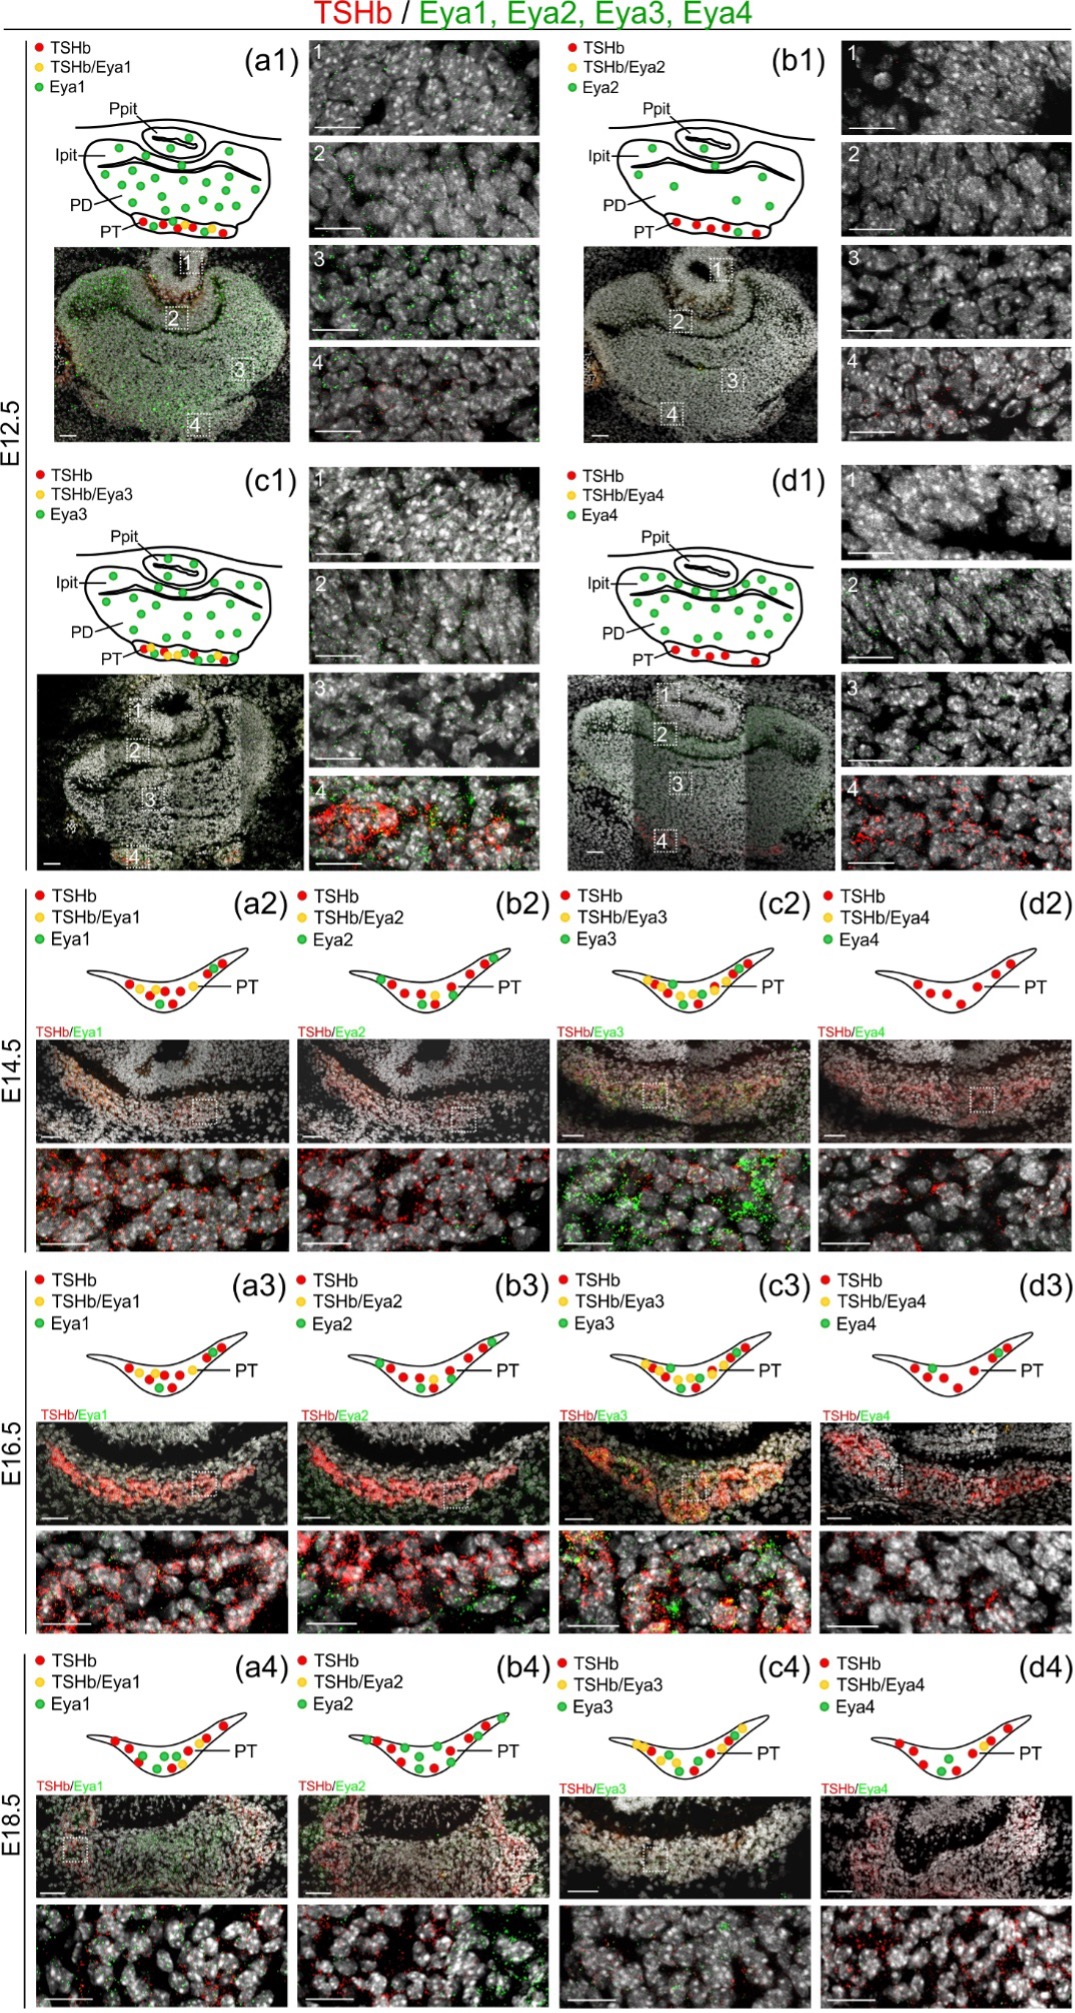
\includegraphics[keepaspectratio]{images/Figure2.jpg}}

}

\caption{\label{fig-fetal-eya-tshb}Localization of \textbf{Tshb} and
\textbf{Eya} transcription coactivators in the fetal PT.}

\end{figure}%

\begin{figure}

\centering{

\pandocbounded{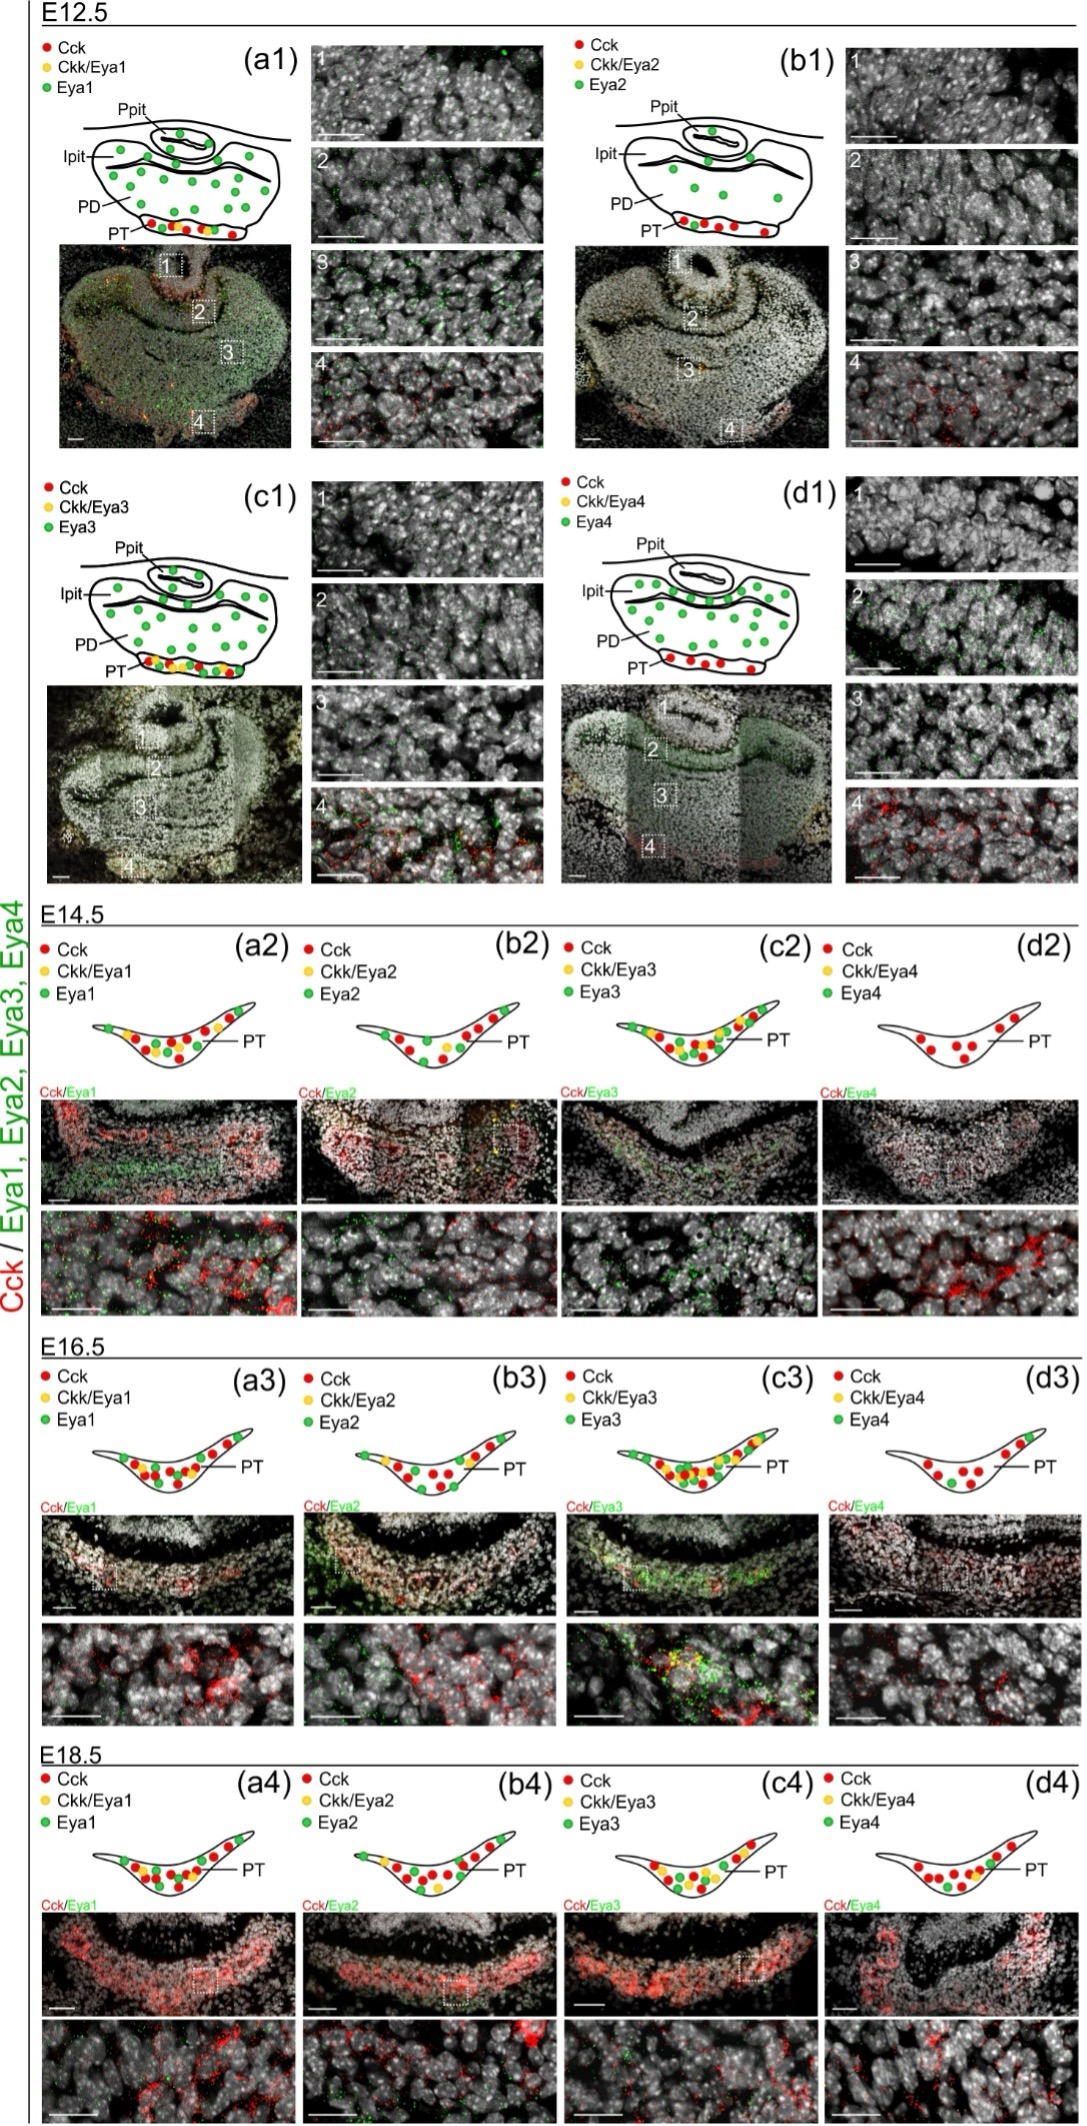
\includegraphics[keepaspectratio]{images/Figure3.jpg}}

}

\caption{\label{fig-fetal-eya-cck}Localization of \textbf{Cck} and
\textbf{Eya} transcription coactivators in the fetal PT.}

\end{figure}%

\begin{figure}

\centering{

\pandocbounded{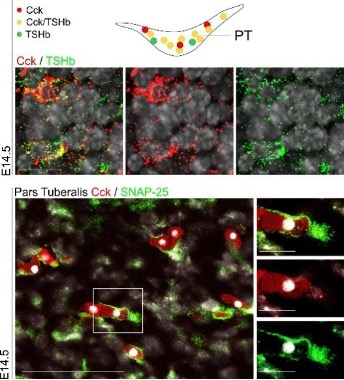
\includegraphics[keepaspectratio]{images/Figure4.jpg}}

}

\caption{\label{fig-fetal-tshb-cck}\textbf{Tshb} and \textbf{Cck}
co-localization.}

\end{figure}%

To further elucidate the characteristics of these groups, we examined
additional genes implicated in PT development and function:

\begin{itemize}
\tightlist
\item
  \textbf{Pitx1 Co-expression}: \emph{Pitx1}, essential for pituitary
  development, was co-expressed with \emph{Eya3} in group one cells
  (Fig. 3a). This co-localization reinforces the idea that group one
  cells are actively involved in hormone production and early PT
  development.
\item
  \textbf{Sox2 Expression}: \emph{Sox2}, a marker of neural stem and
  progenitor cells, was expressed across all PT cell groups (Fig. 3b).
  The presence of \emph{Sox2} suggests that PT cells may share common
  progenitor characteristics or that neural stem cell pathways influence
  PT cell differentiation.
\end{itemize}

We also explored the potential interactions between PT-derived hormones
and the developing brain:

\begin{itemize}
\tightlist
\item
  \textbf{Hormone Receptor Expression}: The receptors for \emph{Tshb}
  (\emph{Tshr}) and \emph{Cck} (\emph{Cckbr}) were expressed in regions
  of the developing hypothalamus rich in neural progenitor cells, such
  as the ventricular zones (Fig. 4a, 4b). Co-expression of \emph{Tshr}
  and \emph{Cckbr} with \emph{Sox2} indicates that PT-derived hormones
  could influence neural development by acting on these progenitor
  cells.
\item
  \textbf{Gpr173 Expression}: We observed expression of \emph{Gpr173}, a
  G protein-coupled receptor involved in neuroendocrine signaling, in
  neural progenitor zones overlapping with \emph{Sox2} expression (Fig.
  4c). This suggests a potential role for \emph{Gpr173} in mediating
  hormonal signals from the PT to the developing brain.
\end{itemize}

\begin{figure}

\centering{

\pandocbounded{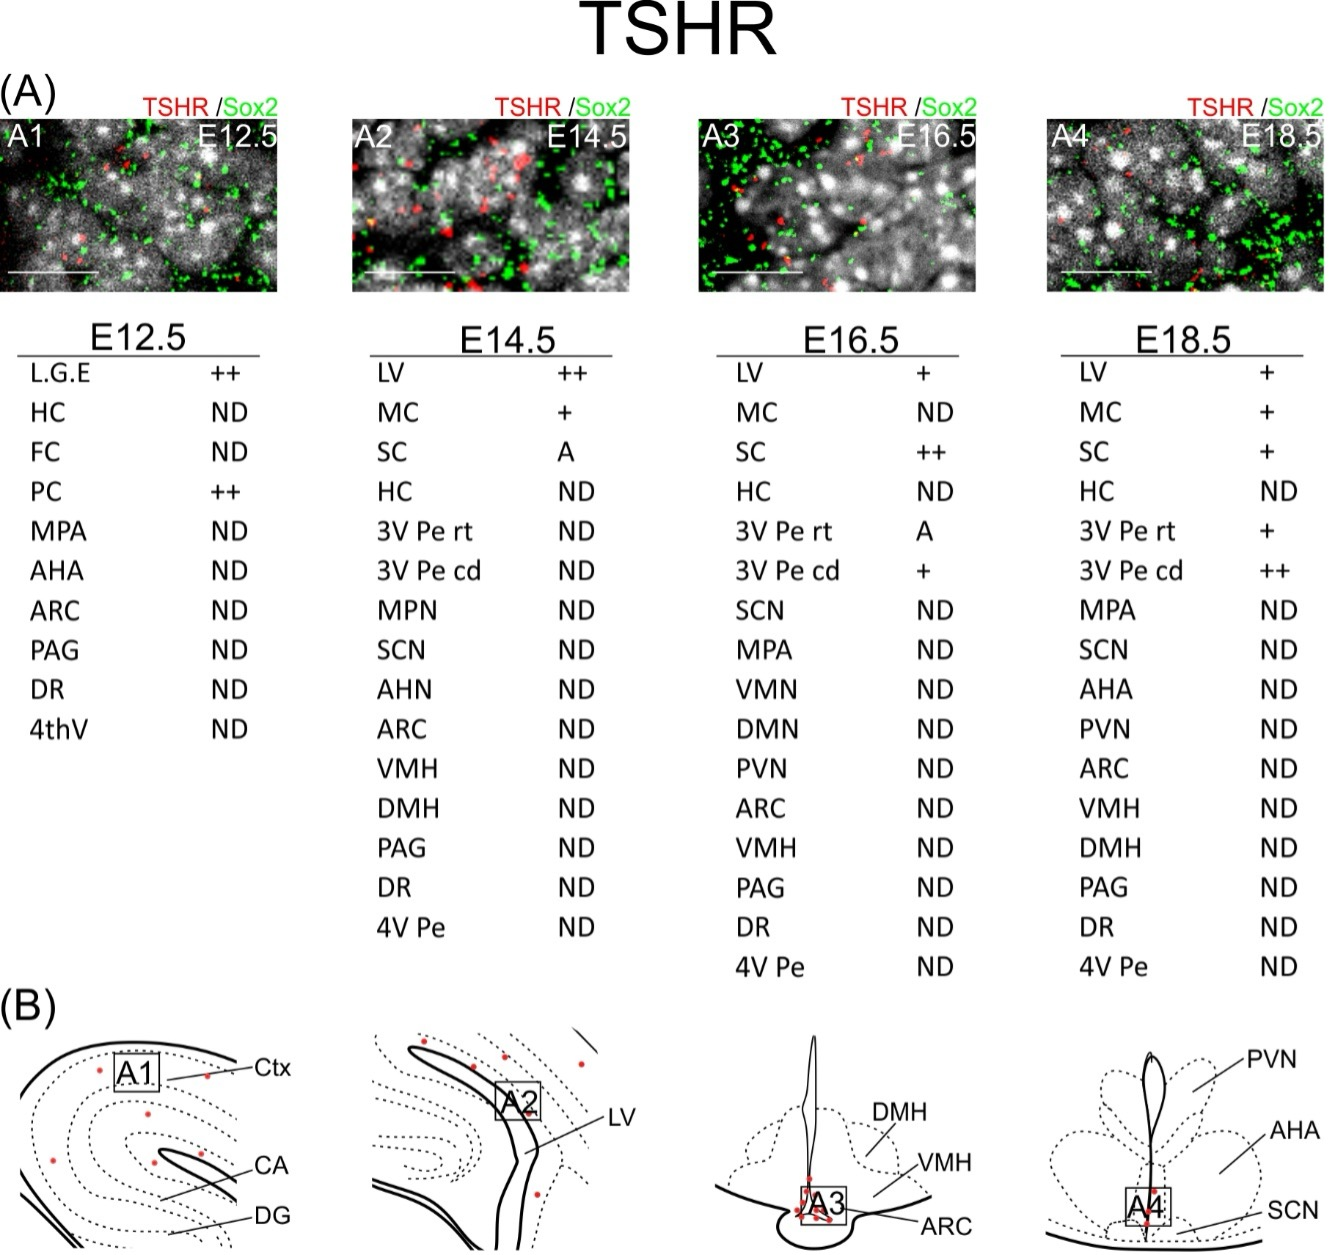
\includegraphics[keepaspectratio]{images/Figure5.jpg}}

}

\caption{\label{fig-fetal-tshr}\textbf{TSHR} brain-wide mRNA
expression.}

\end{figure}%

\begin{figure}

\centering{

\pandocbounded{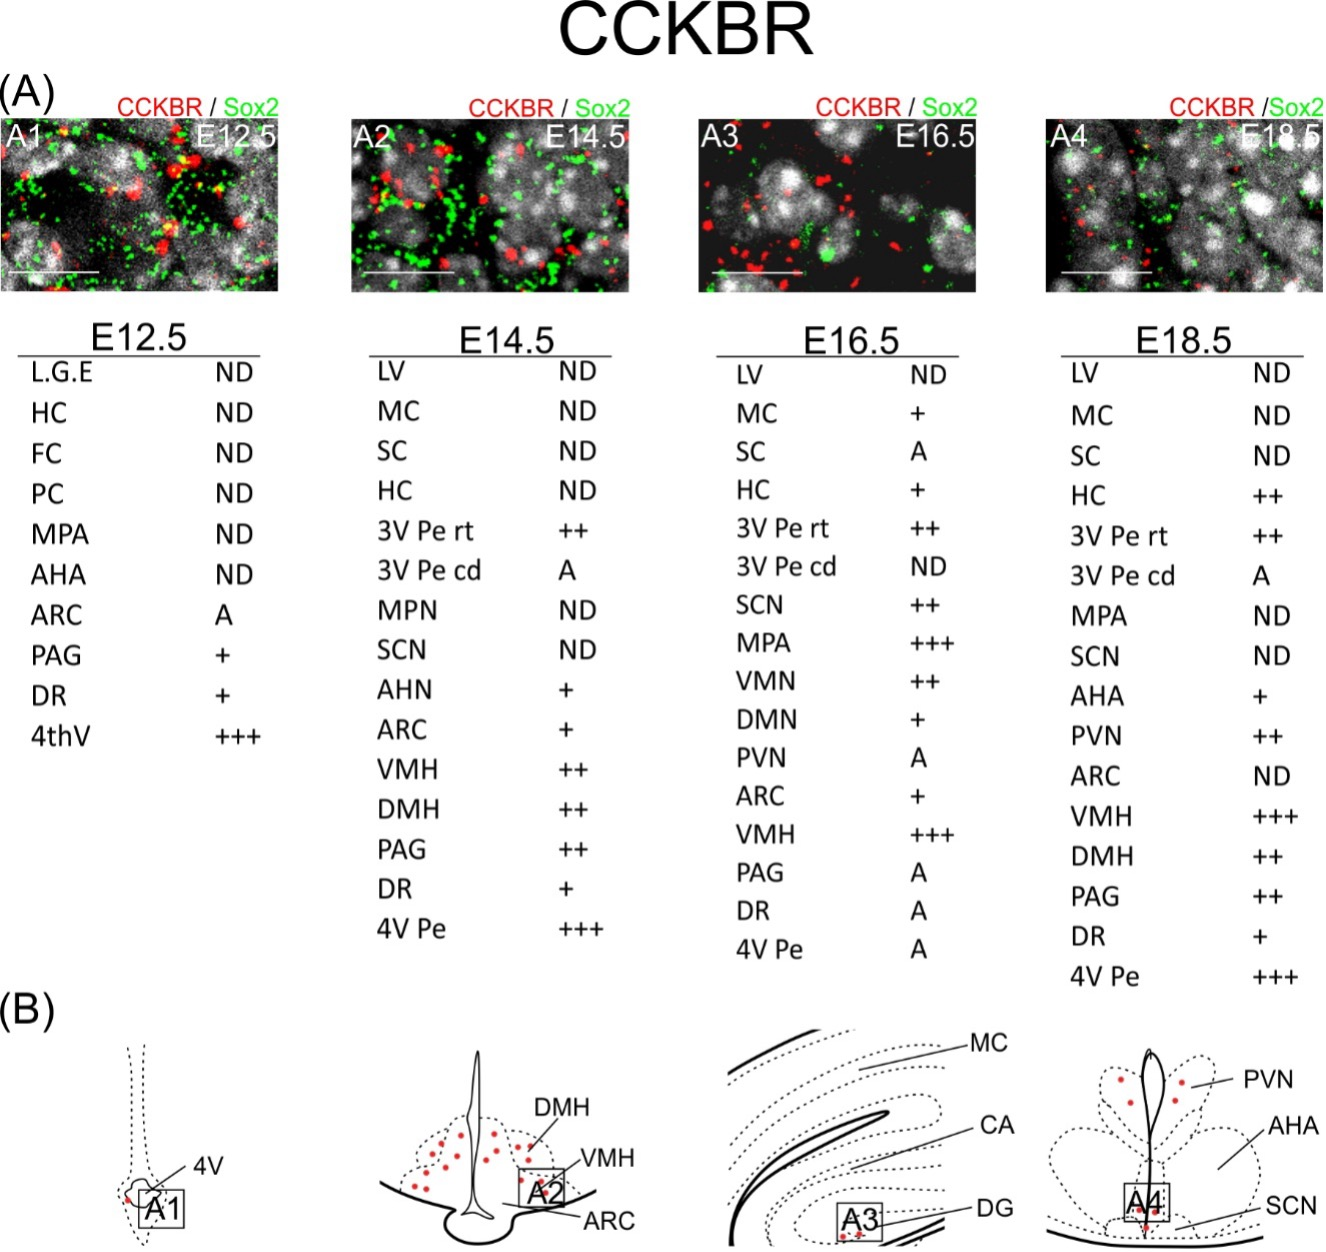
\includegraphics[keepaspectratio]{images/Figure6.jpg}}

}

\caption{\label{fig-fetal-cckbr}\textbf{CCKBR} brain-wide mRNA
expression.}

\end{figure}%

To visualize gene expression dynamics across developmental stages, we
generated DotPlots for key genes (Fig. 5). This analysis highlighted:

\begin{itemize}
\tightlist
\item
  \textbf{Early Onset and Persistence of Group One Genes}: \emph{Eya3},
  \emph{Tshb}, and \emph{Cck} expression began as early as E12 and
  continued throughout embryonic development, indicating a sustained
  role in PT function.
\item
  \textbf{Temporal Emergence of Group Two and Three Genes}: \emph{Eya1},
  \emph{Eya2}, and \emph{Eya4} displayed increased expression at later
  stages, suggesting these genes are involved in the maturation and
  specialization processes within the PT.
\end{itemize}

\begin{figure}[H]

\centering{

\pandocbounded{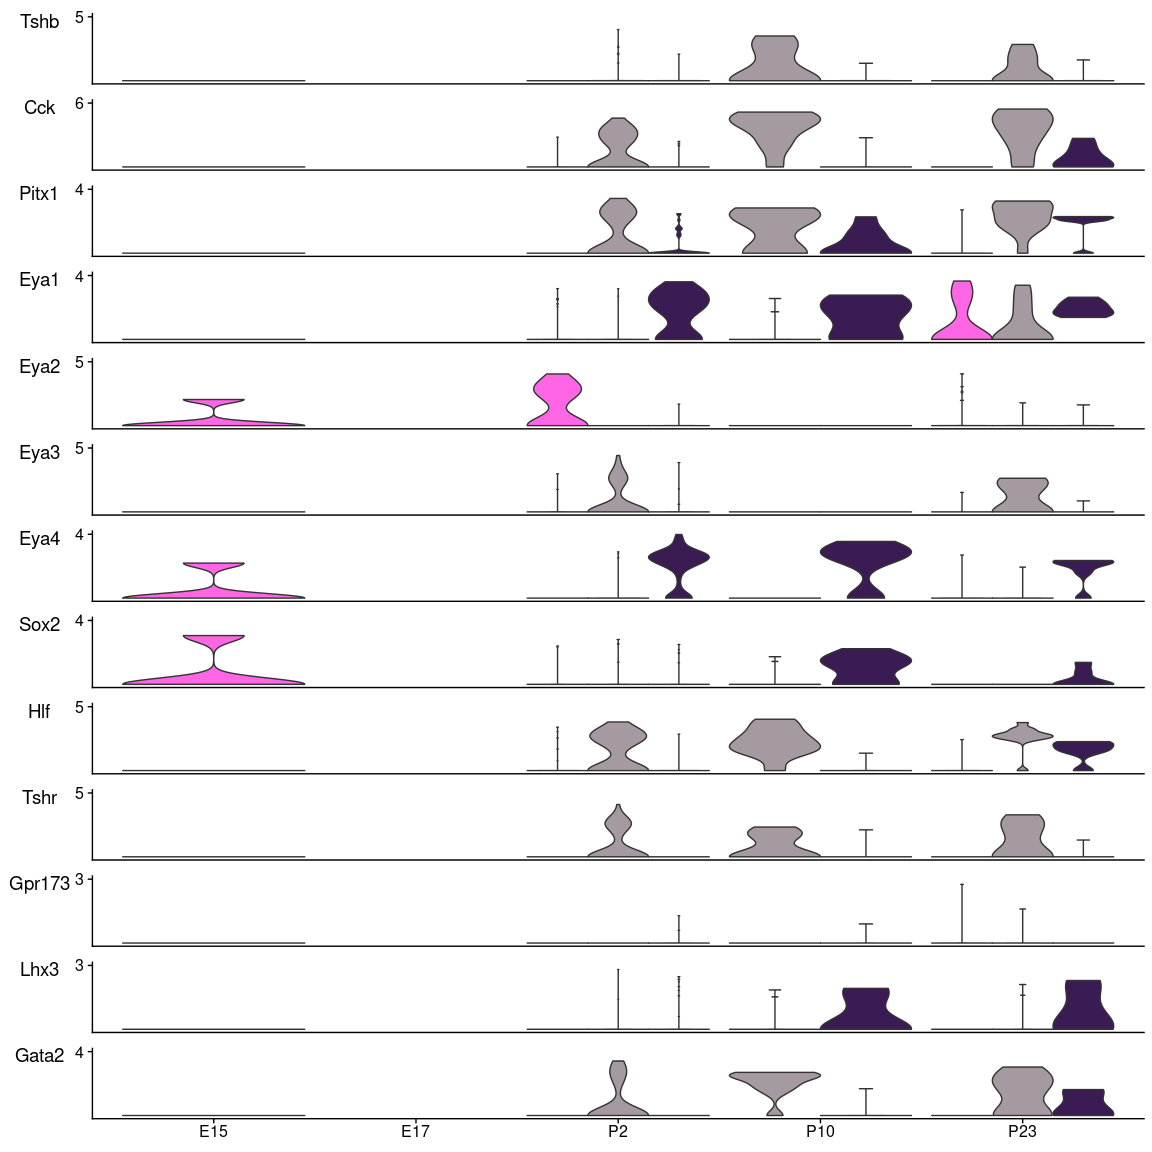
\includegraphics[keepaspectratio]{index_files/figure-latex/notebooks-01-de_test-focus_pars_tub-fig-violin-gene-interactions-romanov2020-output-2.png}}

}

\caption{\label{fig-violin-gene-interactions-romanov2020}Gene expression
of projected Pars Tuberalis clusters in hypothalamus across different
developmental stages in the Romanov et al.~(2020) dataset.}

\end{figure}%

\textsubscript{Source:
\href{https://EugOT.github.io/pr-PT/notebooks/01-de_test-focus_pars_tub.qmd.html\#cell-fig-violin-gene-interactions-romanov2020}{Differential
expression analysis of Hypothalamus datasets from Kim DW}}

Our integrated analysis, combining data from multiple developmental
stages and employing rigorous statistical correlations, provides
compelling evidence for the existence of three distinct PT cell groups
during embryogenesis. Each group exhibits unique transcriptional
signatures, indicating specialized roles:

\begin{itemize}
\tightlist
\item
  \textbf{Group One} is likely responsible for early hormone production,
  directly influencing both PT development and possibly exerting effects
  on the hypothalamus through hormone secretion.
\item
  \textbf{Group Two} may be involved in structural formation or
  regulation within the PT, given their distinct gene expression profile
  and later emergence.
\item
  \textbf{Group Three} could represent a specialized lineage that plays
  a role in the maturation of the PT or has unique endocrine functions.
\end{itemize}

\section{Methods}\label{sec-data-methods}

\subsection{Data Acquisition and
Preprocessing}\label{data-acquisition-and-preprocessing}

Single-cell RNA sequencing (scRNA-seq) data from the mouse hypothalamus
were obtained from the study by Kim et al.\citep{kim2020}, available
under BioProject accession PRJNA547712
(https://github.com/EugOT/PRJNA547712). The dataset, comprising
expression profiles of 128,006 cells across 27,998 genes, was acquired
in the AnnData format (kim2020\_combined.h5ad). This dataset spans
various developmental stages, including embryonic days (E)10 to E18 and
postnatal days (P)4 to P45. To facilitate analysis in R, the AnnData
object was converted into a Seurat
object\citep{haoDictionaryLearningIntegrative2023, stuartComprehensiveIntegrationSingleCell2019}.
The expression matrix was transposed to align genes as rows and cells as
columns. Cell metadata, including identifiers and developmental stages,
were incorporated. Dimensionality reduction was performed using Uniform
Manifold Approximation and Projection
(UMAP)\citep{mcinnes2018, kobakInitializationCriticalPreserving2021},
and the resulting embeddings were added to the Seurat object for
visualization purposes.

\subsection{Integration with Reference
Dataset}\label{integration-with-reference-dataset}

To annotate cell types within the pars tuberalis (PT), we integrated
query dataset\citep{kim2020} with a reference scRNA-seq dataset
(https://github.com/EugOT/PRJNA548917), which provides detailed
annotations of hypothalamic cell
populations\citep{romanovMolecularDesignHypothalamus2020}. The reference
dataset was updated to ensure compatibility and included 51,199 cells
with expression profiles for 24,340 genes.

Anchors between the query dataset\citep{kim2020} and the reference
dataset\citep{romanovMolecularDesignHypothalamus2020} were identified
using the FindTransferAnchors function in
Seurat\citep{haoDictionaryLearningIntegrative2023, stuartComprehensiveIntegrationSingleCell2019},
employing principal component analysis (PCA) for dimensionality
reduction over 30 dimensions. Cell type labels were transferred from the
reference to the query dataset using the TransferData function, allowing
for the prediction of cell identities within the
PT\citep{haoDictionaryLearningIntegrative2023}. The integration
facilitated the identification of specific cell clusters corresponding
to the PT, marked by the expression of genes such as Tshb, Cck, and
Eya3.

\subsection{Normalization and Feature
Selection}\label{normalization-and-feature-selection}

The integrated Seurat object was normalized using the NormalizeData
function, applying global-scaling normalization to account for
differences in sequencing depth. Variable features were identified using
the FindVariableFeatures function with the `vst'
method\citep{hafemeister2019}, selecting the top 3,000 genes exhibiting
high variability across cells. The data were then scaled using the
ScaleData function, regressing out unwanted sources of variation and
centering and scaling the data for downstream analyses.

\subsection{Dimensionality Reduction and
Visualization}\label{dimensionality-reduction-and-visualization}

Principal component analysis was conducted on the scaled data, and the
first 30 principal components were used for further analysis. UMAP was
performed using the RunUMAP function to visualize the data in
two-dimensional space, capturing the global structure and potential
trajectories of cellular differentiation.

Feature plots were generated using the FeaturePlot function to visualize
the expression patterns of key genes across developmental stages. Genes
of interest included Tshb, Cck, Pitx1, Eya1, Eya2, Eya3, Sox2, Hlf,
Tshr, Cckar, Cckbr, and Gpr173. Blended feature plots were employed to
examine co-expression patterns, with parameters adjusted for optimal
visualization (e.g., blend thresholds, point sizes, alpha levels, and
color schemes).

\subsection{Statistical Analysis}\label{statistical-analysis}

To assess the association between the expression of specific genes
across developmental stages, chi-squared tests of independence were
conducted. Binary expression matrices were created by thresholding gene
expression counts (e.g., considering a gene as expressed using
gene-specific quantile thresholding). Contingency tables were
constructed for pairs of genes (\emph{Tshb}, \emph{Cck}, \emph{Pitx1},
\emph{Eya1}, \emph{Eya2}, \emph{Eya3}, \emph{Eya4}, \emph{Sox2},
\emph{Hlf}, \emph{Tshr}, \emph{Cckar}, \emph{Cckbr}, and \emph{Gpr173}),
such as \emph{Sox2} and \emph{Tshr}, across different developmental
stages.

The ggpiestats function from the ggstatsplot package\citep{patil2021}
was utilized to generate grouped pie charts, displaying the proportion
of cells expressing combinations of genes and the results of chi-squared
tests. The analyses provided insights into potential regulatory
relationships and developmental dynamics within the PT.

UpSet plots\citep{conwayUpSetRPackageVisualization2017} were created to
visualize the counts and proportions of cells expressing various
combinations of genes across developmental stages. These plots
illustrated the temporal changes in gene expression and the prevalence
of specific cell populations during development.

\subsection{Gene Expression Correlation
Analysis}\label{gene-expression-correlation-analysis}

To investigate potential co-regulation and interactions between genes,
correlation analyses were performed. Spearman's rank correlation
coefficients were calculated for pairs of genes across cells at each
developmental stage. Hexbin plots were generated using the hexbin
package to visualize the density and correlation of gene expression in a
two-dimensional space, aiding in the identification of spatial
expression patterns and clusters.

Dot plots were generated using the DotPlot function to summarize the
expression of genes of interest across developmental stages. The genes
included \emph{Tshb}, \emph{Cck}, \emph{Pitx1}, \emph{Eya3},
\emph{Sox2}, \emph{Hlf}, \emph{Igfbp5}, \emph{Tshr}, \emph{Cckar},
\emph{Cckbr}, and \emph{Gpr173}. The dot plots represented both the
proportion of cells expressing each gene and the average expression
levels, providing a comprehensive overview of gene expression dynamics
during development.

\subsection{Data Availability}\label{data-availability}

The code (\url{https://github.com/EugOT/pr-PT}) and datasets used in
this study are publicly available. The Kim\citep{kim2020} dataset can be
accessed under BioProject accession PRJNA547712, and the
Romanov\citep{romanovMolecularDesignHypothalamus2020} dataset is
available under BioProject accession PRJNA548917 including repository
with reprocessing code: \url{https://github.com/EugOT/PRJNA547712} and
\url{https://github.com/EugOT/PRJNA548917}.


\renewcommand\refname{References}
  \bibliography{bibliography.bib}



\end{document}
